\chapter{Preparation}
This project involved vast exploratory design work, in preparation of the actual implementation.

	\section{Requirements}
	This project could go in numerous different design directions from the start. Since the functionality and its benefits over existing systems depended heavily on the design chosen, it was hard to separate what benefits the program would achieve from what features the program would include and how it would expose them to the user. 
	
	However, in order to focus our exploration and make sure that the focus was on achieving some real deliverables for end users, a requirement analysis was necessary. The following functional goals were listed based on the project proposal, which focus on what basic tasks the system must help the user achieve, while allowing leeway in how the program exposed and implemented these features.
	
	The system must allow the user to:
	\begin{enumerate}[label=\bfseries Core \arabic*:]
		\item Use any data they have in reasonably arranged formats in common file types.
		\item Specify the type of chart they want by drawing a likeness of it on screen using a stylus.
		\item Bind the data to the chart using an interface that makes it clear how the data is affecting the visualisation.
		\item Specify visual, size and positioning properties of the chart through the sketches.
		\item Manipulate the visual appearance of the created chart.
	\end{enumerate}
	
	In addition, time permitting, the system may:
	\begin{enumerate}[label=\bfseries Extension \arabic*:]
		\item Transform user-drawn sketches to show the visual link to the formal chart elements.
		\item Feed back manipulations applied to the formal layer back to the user drawn sketches, in order to keep the visuals of the formal and sketch layers in synchronisation.
		\item Allow users to undo actions by erasing sketches, and remove the corresponding formal elements without throwing errors.
		\item Allow users to manipulate any property of chart elements, not just one, so that the domain of visualisations they can create is infinite. For example, allow them to bind not just the height of bars in a bar chart to data, but also their width and colour. 
		\item Analyse the data and infer properties that may allow it to automatically suggest properties of the chart, such as which field belongs on which axis, or whether a data series should be log scale or linear scale.
		\item The user must be able to export the chart as a Microsoft Chart object that can be embedded as a dynamic object in Microsoft Office files, not just as a raster image.
	\end{enumerate}
	
	The core of this project focusses on making more usable software, rather than providing additional functionality, compared to existing systems. Hence, some usability goals were also specified:
	\begin{enumerate}[label=\bfseries Usability \arabic*:]
		\item Users must be able to create charts at least as quickly as they can using current systems.
		\item Users must be able to build a mental model of the software's behaviour within 2 uses of it. They should thus be able to accurately predict the consequences of any action taken within the software.
		\item Changes to the information visualisation must occur through directly manipulating the visual representation of the chart, rather than through disconnected User Interface widgets.
		\item The user must be able to easily try out changes to the visualisation, see what that would look like, and undo them if needed.
	\end{enumerate}
	
	\section{Work Items}
	An iterative development process, similar to the Spiral Model was adopted for this project. This allowed early experimentation with and user testing of the various components and different interface designs. The following broad work items were identified as necessary to achieve the objectives above:
	%TODO Maybe insert a picture of my development process here, including the user studies?
	\begin{enumerate}
		\item Assess the various methods to build a classifier for ink recognition, including using the RATA Framework
		\item Run an initial user study to  see how people naturally draw graphs, and also use it to collect training examples for the classifier.
		\item Build a UI that accepts strokes, runs them through the classifier, and shows the user feedback to indicate successful recognition.
		\item Build the UI widget that lets users import their spreadsheets in Microsoft Excel or Comma Separated Value files. It must then expose the various fields detected.
		\item Build the charting component to convert the recognised sketches and the ink into a finished visualisation.
		\item Run a pilot study followed by a user study to evaluate the system.
	\end{enumerate}
	
	\section{Development Environment}
	For this project, the hardware available was a Microsoft Surface Pro (\nth{1} gen), which features the active digitizer screen required for precise inking. Since this machine runs Windows by default, we chose to develop the system using the .NET framework, which has built-in support for Tablet PCs and Ink handling.
	
	As a precaution, insurance was taken out on the machine to ensure quick replacement in case of damage or loss. Additionally, version control was used extensively in the project, to ensure no work was lost. The code for the RATA ink stroke recogniser, described below, was uploaded to a Git repository in collaboration with RATA's authors. The code for this project was then written in a fork of that repository, to allow updates to RATA to be pulled in. The dissertation itself was written in \LaTeX , so that the text files could be versioned in another Git repository. Both repositories were backed up off-site on repository host Bitbucket. The dissertation was also backed up online using file synchronisation software Microsoft OneDrive. 
	
	\section{Building the classifier}	
	Core to the system is an ink recognition component that identifies the chart element (e.g.\ bar, axis) that the user has sketched. This must work above a certain accuracy threshold or the system will prove frustrating to users \citep{Frankish1995}. However, since the project scope included other components too, the time available to build this classifier was limited. Hence, we decided to build a classifier using existing tools rather than implementing one from scratch. 
	
	\subsection{Tools used}
	The digital ink library Microsoft provides includes an ink stroke recognizer. There are a number of other ink recognition tools available, such as \$1, Rubine, PaleoSketch and CALI. However, while these recognizers work well for the recognition tasks they were designed for, the RATA framework is explicitly designed to allow generation of a custom recogniser for a new domain using a few example images \citep{Chang2010}. It thus outperforms a number of these recognisers on data sets other than the examples they ship with. By choosing to use RATA, we ensured we got a high accuracy rate for a domain of chart elements that may need to expand over time to incorporate more types of charts.
	%TODO Do I need to cite a paper introducing each of the named recognisers?
	%TODO Should I include more explanation on why RATA is a great choice compared to the alternatives? This would be largely based on the introduction in the RATA paper cited. This might be restated as evaluating the options we had and how they worked, and seeing that RATA's methodology was best suited for this task.
	
	Rather than using manually specified features and thresholds for these features, RATA uses machine learning to automatically select features and identify relationships between them. It uses the WEKA tool, which provides numerous different data mining algorithms, and combines the results of these algorithms to provide higher accuracy. The authors of RATA also provide a 'Data Manager' tool to facilitate easy collection and labelling of training data. 
	
	\subsection{Data collection}
	After acquiring RATA, we inspected the code and did manual testing to find some blocking bugs. Since we were in contact with the authors of the software, including Beryl Plimmer who until recently worked at the University of Cambridge Computer Lab, we were able to confirm with them that these were indeed bugs. We implemented fixes for them and contributed them back to the authors, and are working towards getting the code ready for to be published Open Source.
	
	With a working version of RATA, an initial study was run to collect training data. We asked 10 participants (20-26 year old Cambridge students, studying a large variety of subjects) to draw a chart. I spoke out the following prompt:
	
	\begin{quotation}
	Imagine you are a government official trying to use a bar chart to visualise how the population has grown over time. Can you sketch out what this bar chart might look like? Just treat this screen like paper.
	\end{quotation}
	
	 They were then presented a simple UI with a large white canvas and the following task description written in a panel:
	
	\begin{quotation}
	Draw 2 axes. Label the x axis 'Year' and the y 'Population'. Draw 3 bars of different heights. Each shape (axis, bar) should be drawn in one stroke.
	\end{quotation}
	
%	First, they were shown a spreadsheet file containing sample data as below:
%	\begin{tabu}{l r r}
%		\rowfont{\bfseries} Year & Births & Deaths \\
%		2010 & 50,000 & 30,000 \\
%		2011 & 40,000 & 35,000 \\
%		2012 & 36,000 & 37,000 \\
%		2013 & 34,000 & 35,000 \\
%	\end{tabu}
%	
%	\vspace{10pt}
%	
%	Next, I spoke out the following task prompt.
%
%	
%	\begin{quote}
%		Say you are a government official trying to visualise trends in birth and death rates over time. Could you draw a bar hart on this screen that you would need to visualise this. No need to plot the actual data, just a rough sketch of what this chart would look like.	
%	\end{quote}
	
	They were asked to draw the same chart 2 times, in order to get 20 training samples in total, and to observe how much variation there is between multiple sketches by the same user. On the second drawing, they were encouraged to draw a less conventional chart, to make the system as robust in the face of variations as possible. 
	%TODO ^Explain this better
		
	\begin{figure}[h]
        \centering
        \begin{subfigure}[b]{0.5\textwidth}
                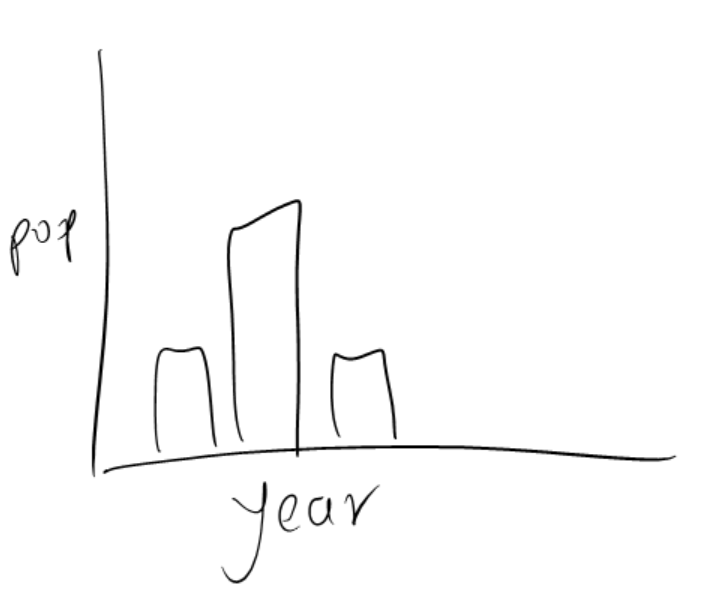
\includegraphics[width=\textwidth]{collection1}
                \caption{Regular chart}
                \label{fig:regular}
        \end{subfigure}%
        ~ %add desired spacing between images, e. g. ~, \quad, \qquad etc.
          %(or a blank line to force the subfigure onto a new line)
        \begin{subfigure}[b]{0.5\textwidth}
                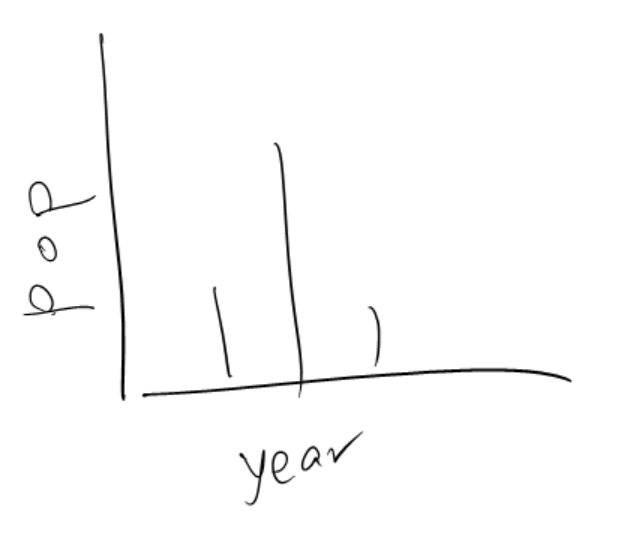
\includegraphics[width=\textwidth]{collection2}
                \caption{Using lines instead of bars}
                \label{fig:lines}
        \end{subfigure}
        ~ %add desired spacing between images, e. g. ~, \quad, \qquad etc.
          %(or a blank line to force the subfigure onto a new line)
          \begin{subfigure}[b]{0.5\textwidth}
                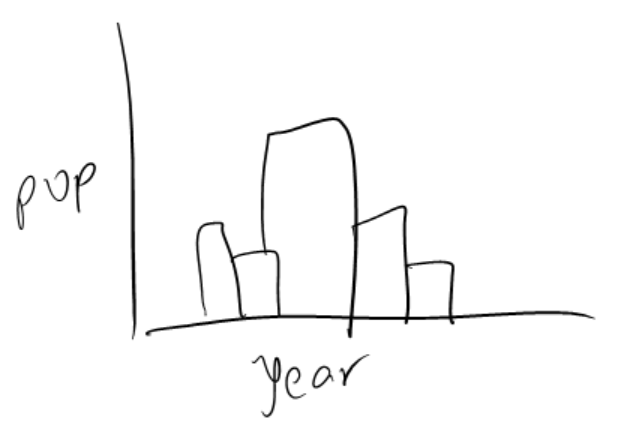
\includegraphics[width=\textwidth]{collection3}
                \caption{Grouped bars}
                \label{fig:grouped}
        \end{subfigure}%
        ~ %add desired spacing between images, e. g. ~, \quad, \qquad etc.
          %(or a blank line to force the subfigure onto a new line)
        \begin{subfigure}[b]{0.5\textwidth}
                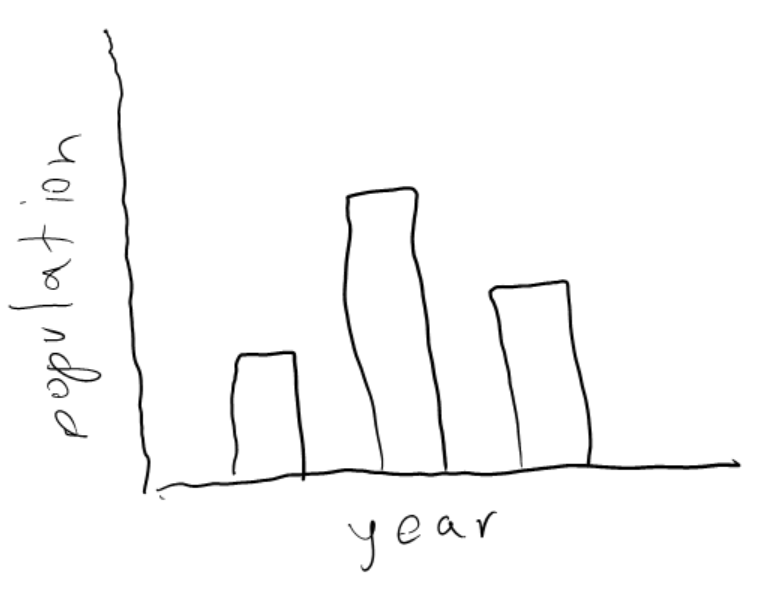
\includegraphics[width=\textwidth]{collection4}
                \caption{Using a mouse instead of the stylus}
                \label{fig:trembling}
        \end{subfigure}
        ~ %add desired spacing between images, e. g. ~, \quad, \qquad etc.
          %(or a blank line to force the subfigure onto a new line)
        \caption{Some of the more unusual chart sketches collected}\label{fig:data_collection_samples}
	\end{figure}
	
	Three elements were then defined: Axis, Bar and Text (an extra element, 'L Axis' was added later based on feedback from a pilot user study). We went through each figure and labelled the various elements.
	
	\begin{figure}[h]
		\centering
		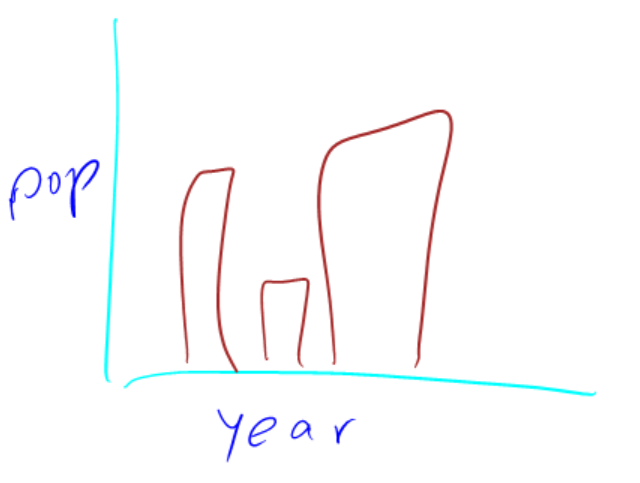
\includegraphics[width=0.5\textwidth]{collection_labelled}
		\caption{Elements of the sketch labelled as Axis (cyan), Bar (brown) or Text (dark blue)}
		\label{fig:collection_labelled}
	\end{figure}

	Once all the elements in all the charts were labelled, we could begin training. RATA includes a dataset generator tool that allowed easy extraction of various features of the strokes, such as 'distance from first to last point', 'absolute curve of largest segment' and 'pressure variation'. This data was compiled into a .csv file for use in training. 
	\subsection{Training}	
	
	\section{Design}
	\section{Planning}
